%
% LaTex file of "User Guide of ARMvisor"
%
% Copyright (c) 2012 SSLab, NTHU
% Author: Peter Chang (phchang@sslab.cs.nthu.edu.tw)
%
% This document and its source code is released under GNU GPLv2 license.
%
% This program is free software; you can redistribute it and/or modify
% it under the terms of the GNU General Public License, version 2, as
% published by the Free Software Foundation.
%
% This program is distributed in the hope that it will be useful,
% but WITHOUT ANY WARRANTY; without even the implied warranty of
% MERCHANTABILITY or FITNESS FOR A PARTICULAR PURPOSE.  See the
% GNU General Public License for more details.
%
% You should have received a copy of the GNU General Public License
% along with this program; if not, write to the Free Software
% Foundation, 51 Franklin Street, Fifth Floor, Boston, MA  02110-1301, USA.
% =================================================================================
% This LaTex file is modified from the template provided by kangxi (http://www.ptt.cc/bbs/NTHU_QFG97/M.1251216359.A.65D.html)
% You can download this template from "http://oz.nthu.edu.tw/~g9771504/Thesis_Example.rar".

\documentclass[12pt]{article}  % 12pt means font size
\usepackage{amsmath, amssymb, amsthm}  % For mathematical symbols
\usepackage[a4paper, top=2.54cm, bottom=2.54cm, left=3.17cm, right=3.17cm]{geometry}  % This is the standard setting of thesis of NTHU. Do not change it.
\usepackage{rotating, booktabs}  % For table-rotating 

\linespread{1.5}  % The linespread is 1.5.

\begin{document}

\begin{titlepage}  % Titlepage
\begin{center}
\Large System Software Lab\\
\Large Department of Computer Science\\
\Large National Tsing Hua University\\
\vspace*{20ex}
\huge User Guide of ARMvisor 1.0\\
\vspace*{35ex}
\Large 2012
\end{center}
\end{titlepage}

\pagenumbering{roman}  % Use roman numbers before the main body.

\tableofcontents  % Table of contents
\newpage

\pagenumbering{arabic}  % Use arabic numbers when the main body starts.

\section{Introduction to ARMvisor}
\subsection{What is ARMvisor}

ARMvisor is a virtual machine on ARM architecture. ARMvisor is based on Kernel-based Virtual Machine. ARMvisor have been developed from 2009. Because ARM architecture doesn’t  support virtualization in hardware instruction set until 2011, ARMvisor is para-virtualized virtual machine.

\begin{figure}[h]  % Put pictures here.
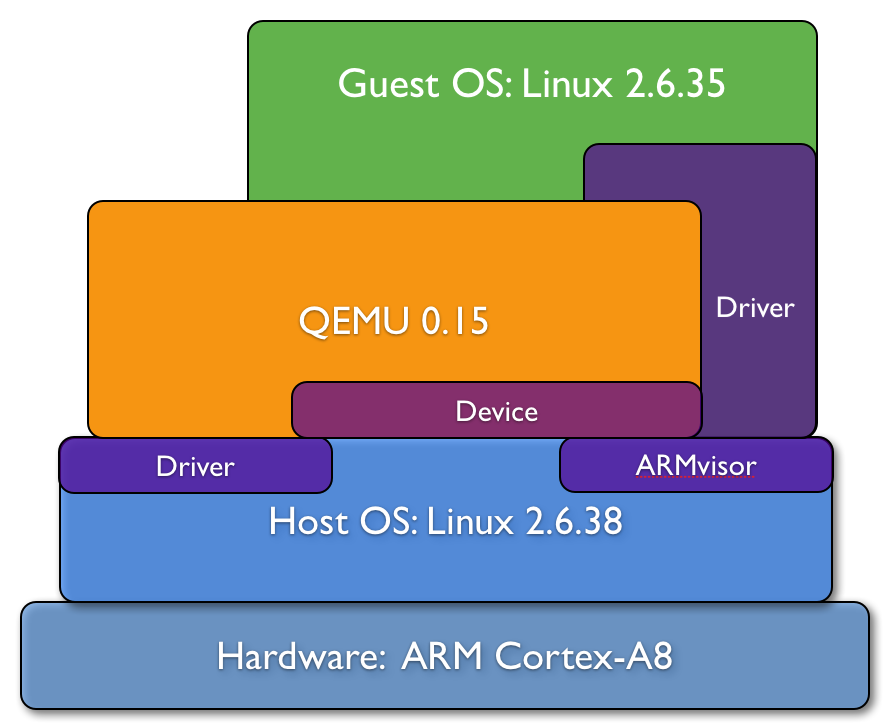
\includegraphics[scale=0.4]{armvisor_archi.png}
\caption{Overview of ARMvisor} 
\label{armvisor_archi}
\end{figure}
In Figure~\ref{armvisor_archi}, we can observe the architecture of ARMvisor. On the bottom, it is ARM-based hardware. Above the hardware, it's Host OS's kernel which include ARMvisor. Because ARMvisor is a part of Linux kernel, if you want to use ARMvisor, you have to use the kernel with ARMvisor. You can use our pre-compiled kernel image which will be introduced in the following section. If you want to compile the kernel by yourself which will also introduced in another following section.

In the user space of host OS, we need to use QEMU to provide the user to create and manage the VM. Besides, QEMU will also emulate I/O device for Guest OS. If you want to use ARMvisor, you have to use the QEMU modified by us. You can use our pre-compiled QEMU image which will be introduced in the following section. If you want to compile modified QEMU by yourself which will also introduced in another following section. Otherwise, if you want to boot the Guest OS, you can need to give QEMU some parameters to run QEMU in KVM mode. You can use your own parameters to boot. You can also choose the script file provided by us. We will introduce how to use our script to boot Guest OS in the following section.

In the Guest OS, you need to use the special kernel which patched by us. Because our model is para-virtualization. You need to use patched kernel of the Guest OS. As a result, if you want to use ARMvisor, you have to use the patched kernel of the Guest OS. You can use our pre-compiled patched kernel image of the Guest OS which will be introduced in the following section. If you want to compile the patched kernel of the Guest OS by yourself which will also introduced in another following section.

\subsection{How to use ARMvisor}

You can run ARMvisor on the most of standard ARMv6/ARMv7 hardware. In following section, 
%we choose two platforms, QEMU and TI BeagleBoard, to show that how to use ARMvisor.
we choose QEMU to show that how to use ARMvisor.

\section{Use ARMvisor on QEMU}
For those who don't have real ARM-based device but still want to use ARMvisor, this section is what you should read!

In this section, we will introduce that how to use QEMU to emulate ARM device on your x86-based PC. Then, we will also show that how to run the pre-compiled host OS on your QEMU on your x86-based PC. Finally, we will introduce that how to put the pre-compiled Guest OS into the root file system of the Host OS and how to run the Guest OS. Just like the Figure~\ref{armvisor_archi_qemu}.

\begin{figure}[h]  % Put pictures here.
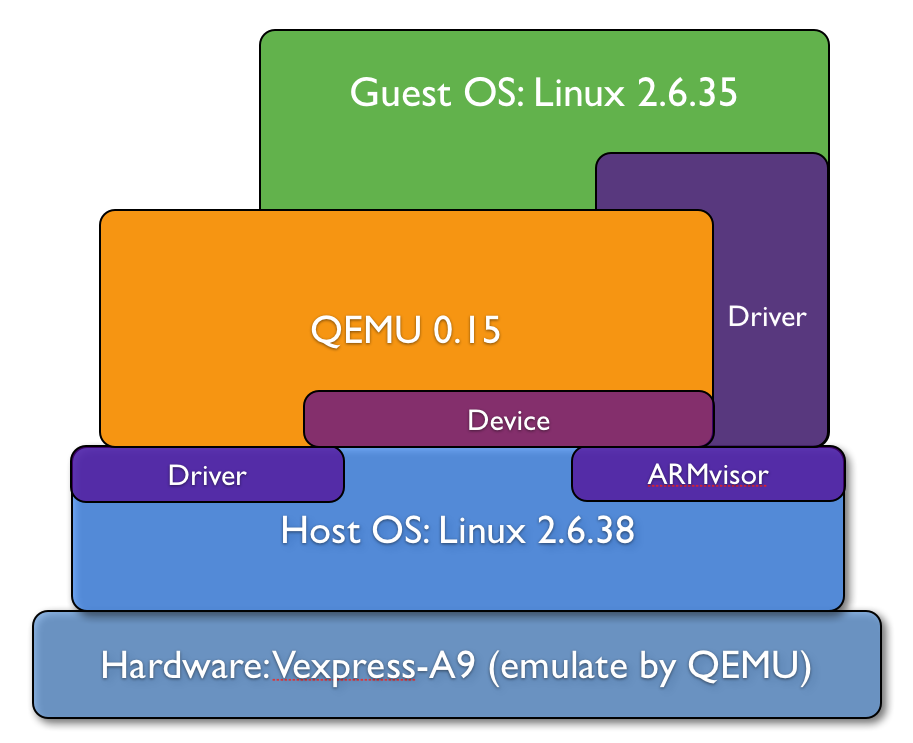
\includegraphics[scale=0.4]{armvisor_archi_qemu.png}
\caption{Overview of ARMvisor in the hardware emulated by QEMU}
\label{armvisor_archi_qemu}
\end{figure}

\subsection{How to use QEMU to run the Host OS?}
QEMU is a tool to emulate ARM device on x86 PC. For those who don't have real ARM-based device but still want to use ARMvisor, QEMU provides you a emulated ARM device running on your PC. In following sections, we will introduce that how to get QEMU and how to use QEMU to run the Host OS.

\subsubsection{How to get QEMU to run the Host OS?}
If you use Ubuntu/Debian on your PC, you could get QEMU from \texttt{apt-get}. If you use Fedora on your PC, you could get QEMU from \texttt{yum}. If your package management system doesn't include QEMU, you can also download the source code from QEMU website (http://wiki.qemu.org/Main\_Page) and compile it by yourself.\newline\newline
For Ubuntu/Debian user:\newline
\fbox{\texttt{\small \$ sudo apt-get install qemu-system}}

\subsubsection{How to get the kernel image of Host OS?}
You can download our pre-compilied kernel image of the Host OS (https://github.com/SSLab-NTHU/linux-host-armvisor/raw/master/arch/arm/boot/zImage).\newline
\fbox{\texttt{\small \$ mkdir \~/armvisor}}\newline
\fbox{\texttt{\small \$ mkdir \~/armvisor/kernel-host}}\newline
\fbox{\texttt{\small \$ cd \~/armvisor/kernel-host}}\newline
\fbox{\texttt{\small \$ wget http://tinyurl.com/93yrxuj}}\newline

\subsubsection{How to get the root file system of Host OS?}
We don't provide the root file system of Host OS for you. You may reference Linaro website (https://wiki.linaro.org/Platform/DevPlatform/Rootfs) to try to build your root file system.  If you want to build your root file system in the way you want, such as reference the Debian website or Fedora website, it is still available.

\subsubsection{How to run the Host OS?}
You can boot the Host OS by setting some parameters of QEMU. You can also the booting script provided by us (https://github.com/SSLab-NTHU/boot-host-script/raw/master/run-host.sh) to boot the Host OS.\newline
\fbox{\texttt{\small \$ cd \~/armvisor/}}\newline
\fbox{\texttt{\small \$ wget https://github.com/SSLab-NTHU/boot-host-script/raw/master/run-host.sh}}\newline
You could modify the script for fitting your demands.

\subsection{Put the Guest OS into the Root File System of the Host OS}
Undoubtedly, the Guest OS, which include its kernel and root file system, needs to be put into the Root File System of the Host OS. Besides, because you need to use modified QEMU to create and manage VM, you also need to put the modified QEMU into the Root File System of the Host OS.

There are several way to put the Guest OS and modified QEMU into the Root File System of the Host OS. You could mount the image file of the Root File System on your PC and put the Guest OS and modified QEMU into the Root File System of the Host OS. You could also use Network File System (a.k.a. NFS) to communicate between the folder on PC and the folder in the Root File System of the Host OS. In the following sections, we will introduce how to get the Guest OS and how to put the Guest OS into the Root File System of the Host OS via NFS.

\subsubsection{How to get the Guest OS?}
You could download the pre-compiled kernel image of the Guest OS from the website ( https://github.com/SSLab-NTHU/linux-guest-armvisor/raw/master/arch/
arm/boot/zImage ).\newline
\fbox{\texttt{\small \$ mkdir \~/armvisor/kernel-guest}}\newline
\fbox{\texttt{\small \$ cd \~/armvisor/kernel-guest}}\newline
\fbox{\texttt{\small \$ wget http://tinyurl.com/9p52286}}

\subsubsection{How to set NFS?}
\begin{enumerate}

\item Before we set up for NFS, we need to install some packages.

\fbox{\texttt{\small \$ sudo apt-get install nfs-kernel-server uml-utilities}}

\item Download the Script provided by us

QEMU will create the script file called as ``qemu-ifup'' and ``qemu-ifdown'' in \texttt{/etc}. When QEMU is executed and want to access network, QEMU will execute this script file. We can use this file to modify the network setting of QEMU.

You could download script codes provided by us from the website ( \newline https://github.com/SSLab-NTHU/qemu-net-script/raw/master/qemu-ifup\newline and https://github.com/SSLab-NTHU/qemu-net-script/raw/master/qemu-ifdown ).

\fbox{\texttt{\small \$ cd \~/armvisor}}

\fbox{\texttt{\small \$ wget http://tinyurl.com/99qf44m}}

\fbox{\texttt{\small \$ wget http://tinyurl.com/8t2sz3y}}

You need to change these scripts' mode into executable and use them to replace ordinary one.

\fbox{\texttt{\small \$ sudo chmod u+x qemu-ifup}}

\fbox{\texttt{\small \$ sudo chmod u+x qemu-ifdown}}

\fbox{\texttt{\small \$ sudo mv qemu-ifup /etc/}}

\fbox{\texttt{\small \$ sudo mv qemu-ifdown /etc/}}

\item Set up the NFS
So far, we have everything that we need to use NFS. We just only have to modify some configurations. We will create a folder which can be accessed by NFS server. Meanwhile, we will also set up the network to let that the network subsystem of the Ubuntu on PC can accept the connection from QEMU.

\begin{enumerate}
\item Create a folder as the NFS folder

\fbox{\texttt{\small \$ mkdir \~/armvisor/nfs}}

\item Add the following words into \texttt{/etc/exports}

\fbox{\small{/home/username/armvisor/nfs 192.168.16.0/24(rw,async,no\_root\_squash,no\_subtree\_check)}}
\fbox{\small{/home/username/armvisor/nfs localhost(rw,async,no\_root\_squash,no\_subtree\_check)}}

\item Add the following words into \texttt{/etc/hosts.allow} to open the connection for NFS

\fbox{\small{nfsd:ALL
portmap:ALL
mountd:ALL}}

\item Let NFS server reload the configuration

\fbox{\texttt{\small \$ sudo /etc/init.d/portmap restart}}

\fbox{\texttt{\small \$ sudo /etc/init.d/nfs-kernel-server restart}}

\end{enumerate}

\end{enumerate}

\subsubsection{Put the Guest OS into NFS folder}
\begin{enumerate}
\item Change directory into the NFS folder

\fbox{\texttt{\small \$ cd \~/armvisor/nfs}}

\item Download the pre-compiled modified QEMU for running the Guest OS 

You can get the pre-compiled modified QEMU from the website ( https://github.com/SSLab-NTHU/qemu-guest-armvisor/raw/master/arm-softmmu/qemu-system-arm ).

\fbox{\texttt{\small \$ cd \~/armvisor/nfs}}

\fbox{\texttt{\small \$ wget http://tinyurl.com/8bhuwtq}}

\fbox{\texttt{\small \$ mv 8bhuwtq qemu-system-arm}}

\item Download the pre-compiled kernel image of the Guest OS

\fbox{\texttt{\small \$ cd \~/armvisor/nfs}}

\fbox{\texttt{\small \$ wget http://tinyurl.com/9p52286}}

\fbox{\texttt{\small \$ mv 9p52286 zImage-guest}}

\item Write a booting script for running the Guest OS

Use \texttt{vim} to create ``run-guest.sh'' which include the words in below:

\fbox{\small sudo qemu-system-arm -M realview-eb -cpu arm1136 -kernel zImage-guest -initrd guestfs.gz \\}
\fbox{\small -nographic -enable-kvm -append "console=ttyAMA0"}

Then change its mode into executable

\fbox{\texttt{\small \$ chmod u+x run-guest.sh}}

\end{enumerate}


\subsection{Run the Host OS and Guest OS}

\begin{enumerate}

\item Run the Host OS

\fbox{\texttt{\small \$ cd \~/armvisor}}

\fbox{\texttt{\small \$ ./run-host.sh}}

\item Mount NFS folder

After the host has already been in the shell, you can mount the NFS folder to get the files of the Guest OS

\fbox{\texttt{\small \$ mount -t nfs 192.168.16.1:/home/username/armvisor/nfs /mnt}}

\item Run the Guest OS

\fbox{\texttt{\small \$ cd /mnt}}

\fbox{\texttt{\small \$ ./run-guest.sh}}

\end{enumerate}

%\section{Use ARMvisor on TI BeagleBoard}
%\subsubsection{Hardware environment}
%\begin{itemize}
%\item Host PC: Linux operating system running on x86 PC (in following description, we will use Ubuntu as our host OS)
%\item Target board: TI Beagleboard
%\item Serial cable: a RS232 cable (or you could also use RS232-USB converter cable)
%\item USB keyboard and mouse
%\item (optional)  LCD monitor with DVI port (if you want to output to LCD monitor)
%\end{itemize}


\section{Build source codes by yourself}

\subsection{Prerequisites}
Before you want to build ARMvisor by yourself, you should make sure that you have all necessary environment.

\subsubsection{Software environment}
\begin{itemize}
%\item Dterm/miniCom/Putty on ``host PC''
\item Toolchain binary files (You can get it from \texttt{apt-get})
\item Patched QEMU source code (You can download it from our GitHub site)
\item Host OS kernel source code: Patched Linux kernel source code with ARMvisor (You can download it from our GitHub site)
\item Guest OS kernel source code: Patched Linux kernel source code (You can download it from our GitHub site)
%\item QEMU prerequisites:
%\begin{itemize}
%\item "zlib" libraries and headers
%\item "SDL" libraries and headers
%\item "alsa" libraries and headers (optional "alsa" support: disabel by default but can be enabled with --enable-alsa)
%\item "gnutls" libraries and headers (optional VNC TLS support: enabled by default but can be disabled with --disable-vnc-tls)
%\end{itemize}
\end{itemize}

%On Ubuntu/Debian system, you can install QEMU prerequisites with:

%\fbox{\texttt{\small \$ sudo apt-get install gcc libsdl1.2-dev zlib1g-dev libasound2-dev}}

%\fbox{\texttt{\small \$ sudo apt-get install linux-kernel-headers pkg-config}}

%\fbox{\texttt{\small \$ sudo apt-get install libgnutls-dev libpci-dev}}

\subsection{How to build ARMvisor by yourself}

\subsubsection{How to install and use the toolchain}
If you use Ubuntu, it's quiet easy to get the toolchain. You just use the \texttt{apt-get} to get it.\newline\newline
\fbox{\texttt{\small \$ apt-get install gcc-arm-linux-gnueabi}}

\subsubsection{How to build your Host OS kernel image with ARMvisor from source code}

Before you want to build kernel images by yourself, you should make sure that you have already downloaded the patched host kernel source code.

\begin{enumerate}
\item Please clone \texttt{linux-host-armvisor} by ``git''. In this document, we will clone the repository in ``\texttt{\~/armvisor/src}'' folder.
\begin{enumerate}
\item Change into the directory\newline
\fbox{\texttt{\small \$ mkdir \~/armvisor/src}}\newline
\fbox{\texttt{\small \$ cd \~/armvisor/src}}\newline

\item Clone the source code from GitHub\newline
\fbox{\texttt{\small \$ git clone https://github.com/SSLab-NTHU/linux-host-armvisor.git}}

\end{enumerate}

\item Change default cross-compiler to the cross-compiler provided by us in Makefile
\begin{enumerate}

\item Open the Makefile

\fbox{\texttt{\small \$ cd \~/armvisor/src/linux-host-armvisor}}

\fbox{\texttt{\small \$ vim Makefile}}

\item Search the keyword: ``CROSS\_COMPILE''

\item Change default cross-compiler to ``arm-linux-gnueabi''

\fbox{\texttt{\small CROSS\_COMPILE   ?= arm-linux-gnueabi-}}

\item Save and quit ``Makefile''

\end{enumerate}

\newpage
\begin{figure}[h]  % Put pictures here.
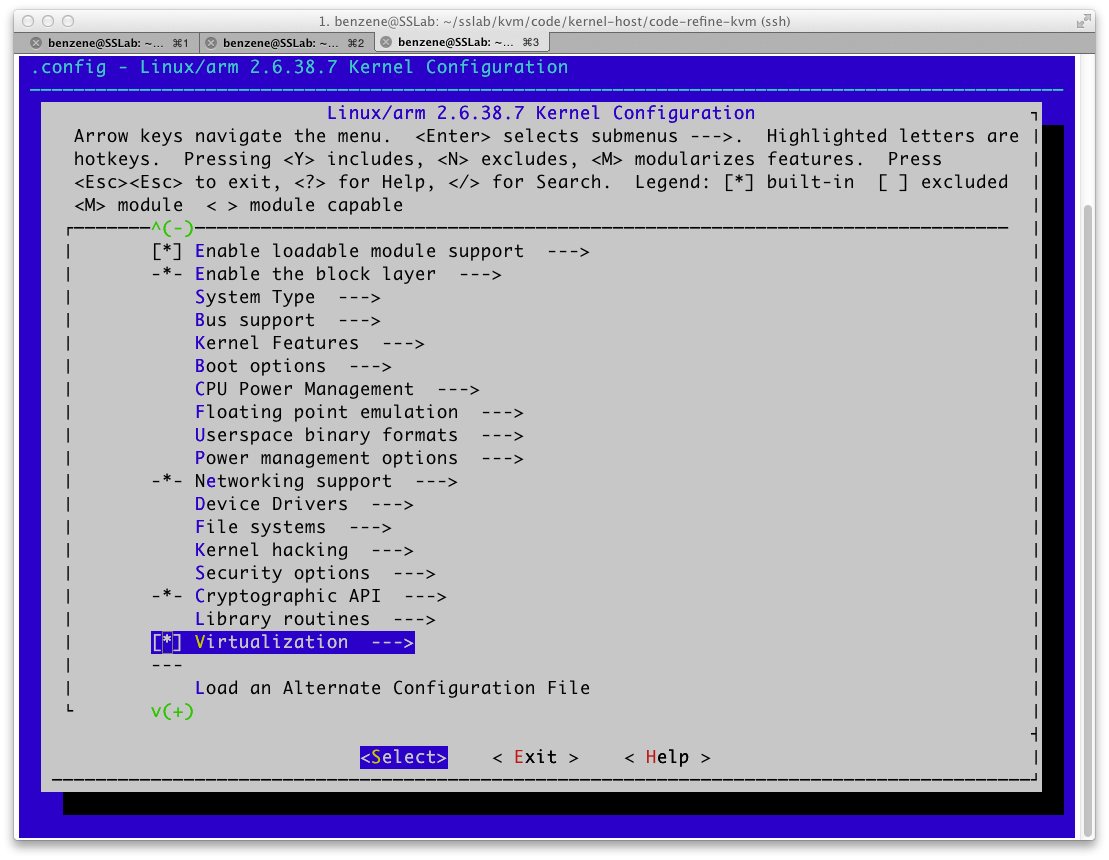
\includegraphics[scale=0.36]{host_menuconfig.png}
\caption{The menuconfig of the Host OS} 
\label{host_menuconfig}
\end{figure}

\item Change directory into linux-host-armvisor, then load default configuration ``config-vexpressa9-armvisor''. You will get the basic environment setting provided by us for Versitile Express A9. The basic environment setting can let you run Linux kernel with ARMvisor.
\begin{enumerate}
\item Use default configuration provided by us\newline
\fbox{\texttt{\small \$ cd \~/armvisor/src/linux-host-armvisor}}\newline
\fbox{\texttt{\small \$ cp config-vexpressa9-armvisor .config}}

\item If you want to change some configs by yourself, you can \texttt{make menuconfig} to modify configs by yourself.


\begin{enumerate}
\item Menuconfig


In Figure~\ref{host_menuconfig}, you can see that we have added a new configuration label, called ``Virtualization'' in menuconfig. We have opened it in the default configuration provided by us. If you want to use ARMvisor, PLEASE DO NOT TURN IT OFF!

\item Optimization

In Figure~\ref{host_menuconfig_opt}, you can see that we provide several optimization flag for you. These optimization can provide tremendous speed-up. However, if you open the optmization flag in the kernel of the Host OS, YOU HAVE TO OPEN THE SAME FLAG WHEN COMPILING THE KERNEL OF THE GUEST!

\begin{figure}[h]  % Put pictures here.
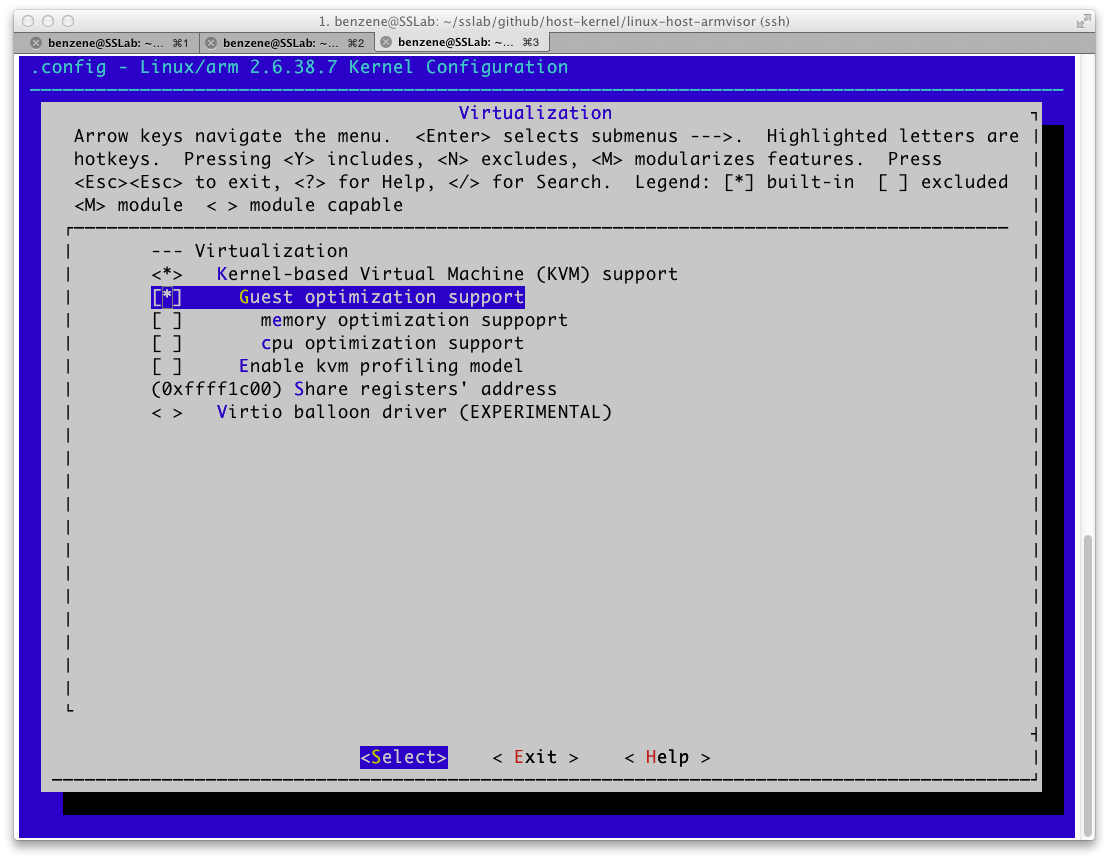
\includegraphics[scale=0.36]{host_menuconfig_opt.png}
\caption{The Optimization configs in menuconfig of the Host OS} 
\label{host_menuconfig_opt}
\end{figure}

\end{enumerate}

\item Make
After ``\texttt{make}'' has been finished, you could find the zImage file in ``\texttt{arch/arm/boot/zImage}''

\fbox{\texttt{\small \$ make -j8}}

\end{enumerate}

%Only for TI BeagleBoard
%\item Before you build your own kernel, you need to install the tool, ``uboot-mkimage'', to help you build your kernel image.\newline
%\fbox{\texttt{\small \$ sudo apt-get install uboot-mkimage}}

%Only for TI BeagleBoard
%\item After you have installed the tool, you can build your own host kernel. It will take you lots of time.\newline
%\fbox{\texttt{\small \$ make uImage}}

\item When it is finished, you will find your kernel image in ``\~/armvisor/src/linux-host-armvisor/arch/arm/boot/zImage''

\end{enumerate}

\subsubsection{How to build the QEMU which is for booting the Guest OS?}
blah

\begin{enumerate}
\item Please clone \texttt{linux-guest-armvisor} by ``git''. In this document, we will clone the repository in ``\texttt{\~/armvisor/src}'' folder.

\begin{enumerate}
\item Change into the directory\newline
\fbox{\texttt{\small \$ cd  \~/armvisor/src}}

\item Clone the source code from GitHub\newline
\fbox{\texttt{\small \$ git clone https://github.com/SSLab-NTHU/qemu-guest-armvisor.git}}

\end{enumerate}

\item Compile it by the script provided by us

\begin{enumerate}
\item Change into the directory\newline
\fbox{\texttt{\small \$ cd  \~/armvisor/src/qemu-guest-armvisor}}

\item Change the mode of the script file\newline
\fbox{\texttt{\small \$ chmod u+x configure-kvm.sh}}

\item Use the script file to set up the configuration\newline
\fbox{\texttt{\small \$ ./configure-kvm.sh}}

\item Compile\newline
\fbox{\texttt{\small \$ make}}

\end{enumerate}

You can find the binary file in the ``\texttt{arm-softmmu/qemu-system-arm}''.

\end{enumerate}

\subsubsection{How to build the kernel image of the Guest OS?}

\begin{enumerate}
\item Please clone \texttt{linux-guest-armvisor} by ``git''. In this document, we will clone the repository in ``\texttt{\~/armvisor/src}'' folder.
\begin{enumerate}
\item Change into the directory\newline
\fbox{\texttt{\small \$ cd  \~/armvisor/src}}

\item Clone the source code from GitHub\newline
\fbox{\texttt{\small \$ git clone https://github.com/SSLab-NTHU/linux-guest-armvisor.git}}

\end{enumerate}

\item Change default cross-compiler to the cross-compiler provided by us in Makefile
\begin{enumerate}

\item Open the Makefile

\fbox{\texttt{\small \$ cd \~/armvisor/src/linux-guest-armvisor}}

\fbox{\texttt{\small \$ vim Makefile}}

\item Search the keyword: ``CROSS\_COMPILE''

\item Change default cross-compiler to ``arm-linux-gnueabi''

\fbox{\texttt{\small CROSS\_COMPILE   ?= arm-linux-gnueabi-}}

\item Save and quit ``Makefile''

\end{enumerate}

\begin{figure}[h]  % Put pictures here.
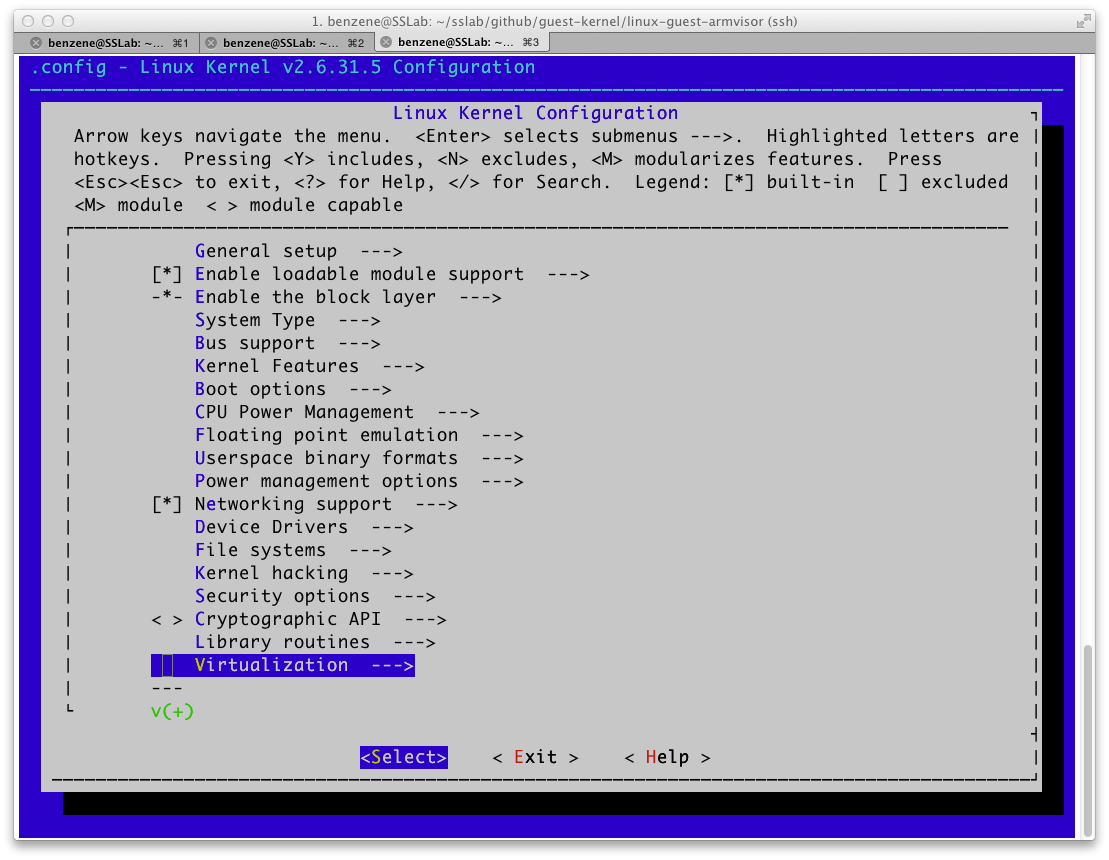
\includegraphics[scale=0.36]{guest_menuconfig.png}
\caption{The menuconfig of the Guest OS} 
\label{host_menuconfig}
\end{figure}
\newpage

\item Change directory into linux-guest-armvisor, then load default configuration ``config-guest-armvisor''. You will get the basic environment setting provided by us. The basic environment setting can let you run Linux kernel with ARMvisor.
\begin{enumerate}
\item Use default configuration provided by us\newline
\fbox{\texttt{\small \$ cd \~/armvisor/src/linux-guest-armvisor}}\newline
\fbox{\texttt{\small \$ cp config-guest-armvisor .config}}


\item If you want to change some configs by yourself, you can \texttt{make menuconfig} to modify configs by yourself.


\begin{enumerate}
\item Menuconfig

In Figure~\ref{host_menuconfig}, you can see that we have added a new configuration label, called ``Virtualization'' in menuconfig. If you want to open the optimization, go into the ``Virtualization'' label.

\item Optimization

In Figure~\ref{guest_menuconfig_opt}, you can see that we provide several optimization flag for you. These optimization can provide tremendous speed-up. However, if you open the optmization flag in the kernel of the Guest OS, YOU HAVE TO OPEN THE SAME FLAG WHEN COMPILING THE KERNEL OF THE HOST!

\begin{figure}[h]  % Put pictures here.
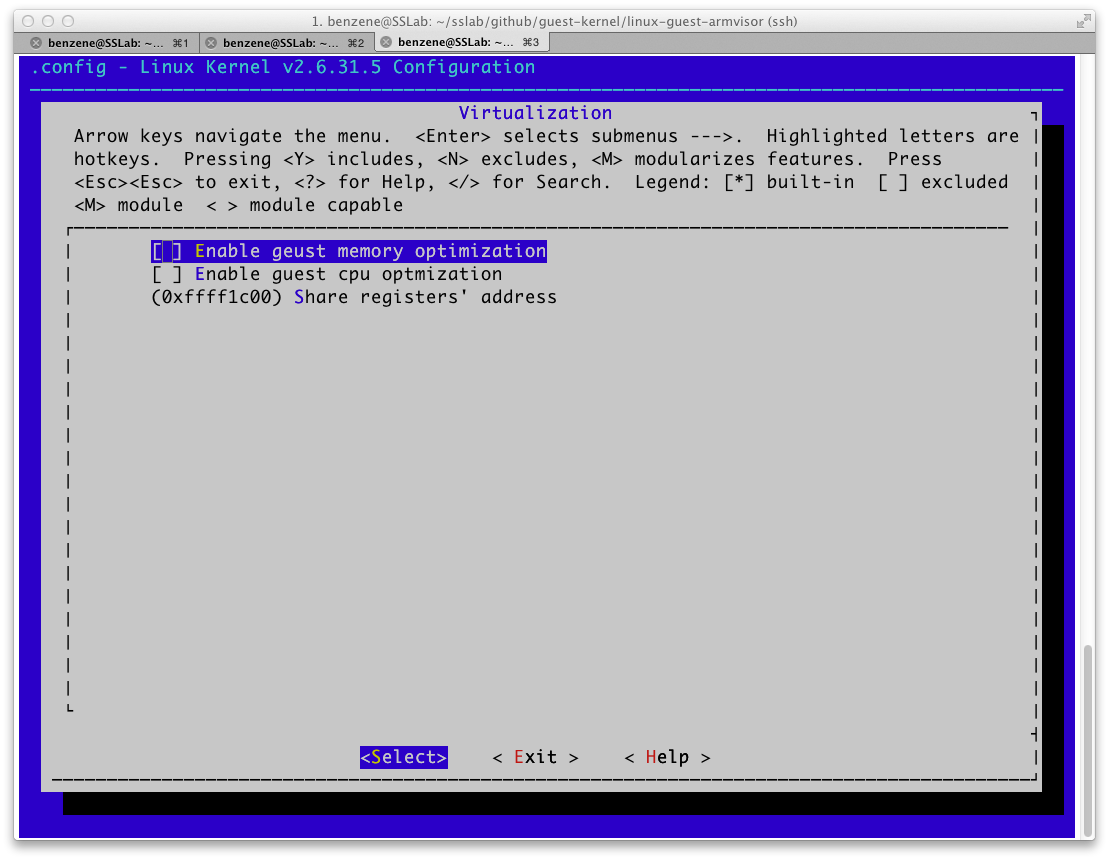
\includegraphics[scale=0.36]{guest_menuconfig_opt.png}
\caption{The Optimization configs in menuconfig of the Guest OS} 
\label{guest_menuconfig_opt}
\end{figure}
\newpage

\end{enumerate}

\item Make
After ``\texttt{make}'' has been finished, you could find the zImage file in ``\texttt{arch/arm/boot/zImage}''

\fbox{\texttt{\small \$ make -j8}}

\end{enumerate}

\end{enumerate}

\end{document} 
